\begin{frame}{Next Generation Sequencing}
     \begin{textblock}{9.2}(1,3)
         \begin{mdframed}[backgroundcolor=white]
            \begin{center}
                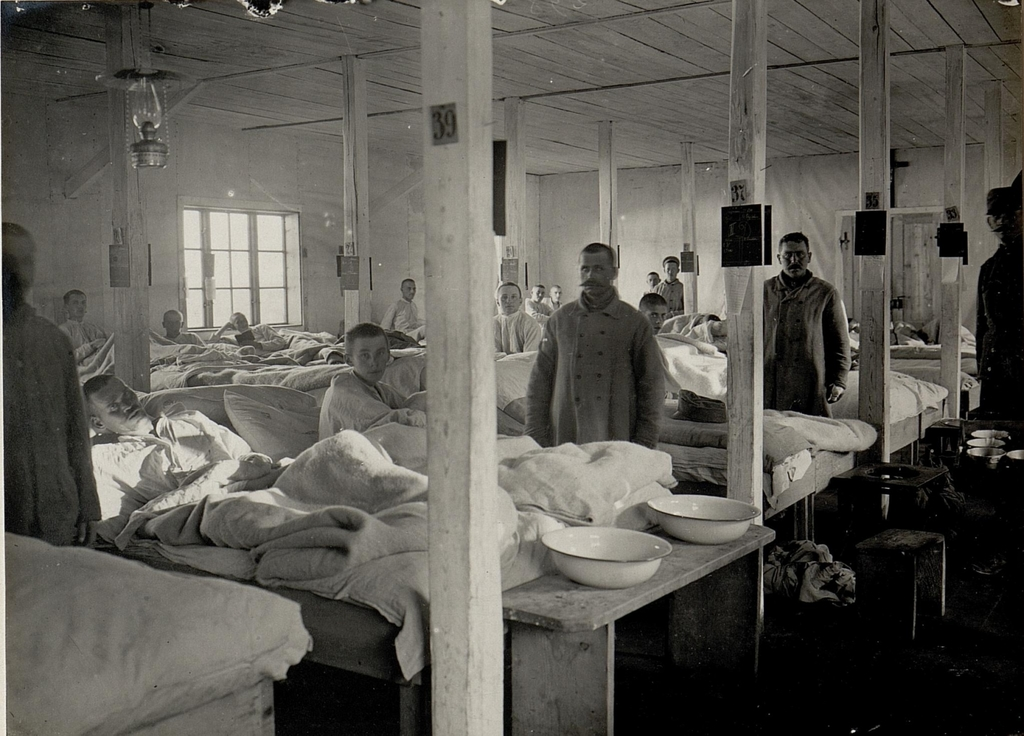
\includegraphics[height=5.3cm]{Kapitel/NGSMotivation/Bilder/typhus_illness.jpg}\\
                \vspace{0.3cm}\captionof{figure}{Typhuszimmer 1916 \cite{typhus_illness}}
            \end{center}
        \end{mdframed}
    \end{textblock}
    \only<2->{
        \begin{textblock}{9.2}(2,3.1)
            \begin{mdframed}[backgroundcolor=white]
                \begin{center}
                    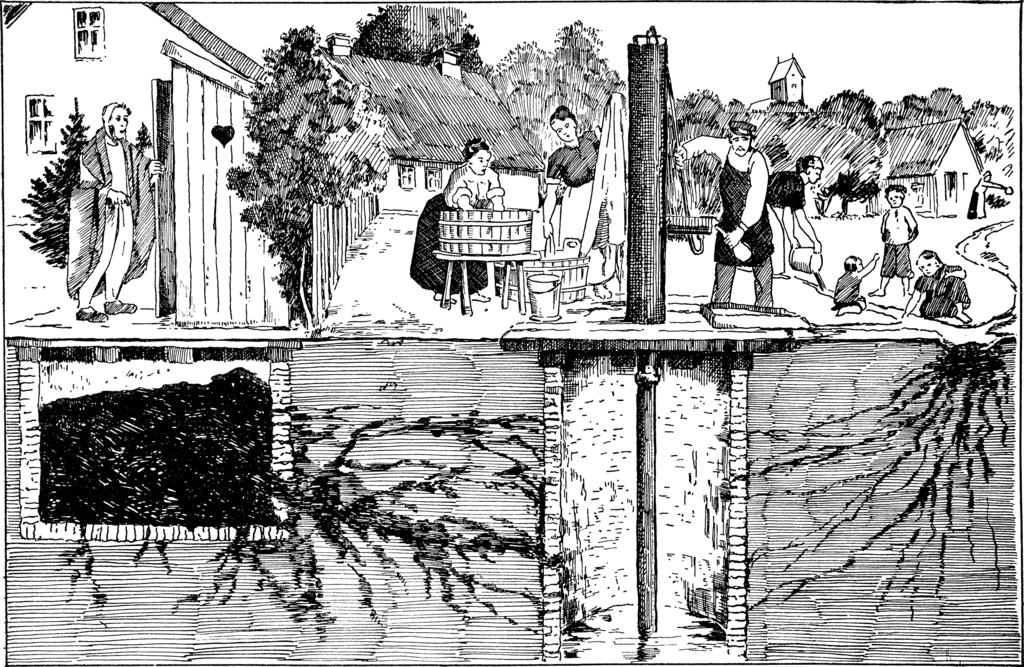
\includegraphics[height=5.3cm]{Kapitel/NGSMotivation/Bilder/typhus_spread.png}\\
                    \vspace{0.3cm}\captionof{figure}{Visualisierung der Typhusverbreitung in einem Buch von 1939 \cite{typhus_spread}}
                \end{center}
            \end{mdframed}
        \end{textblock}
    }
    \only<3->{
        \begin{textblock}{9.2}(3,3.2)
            \begin{mdframed}[backgroundcolor=white]
                \begin{center}
                    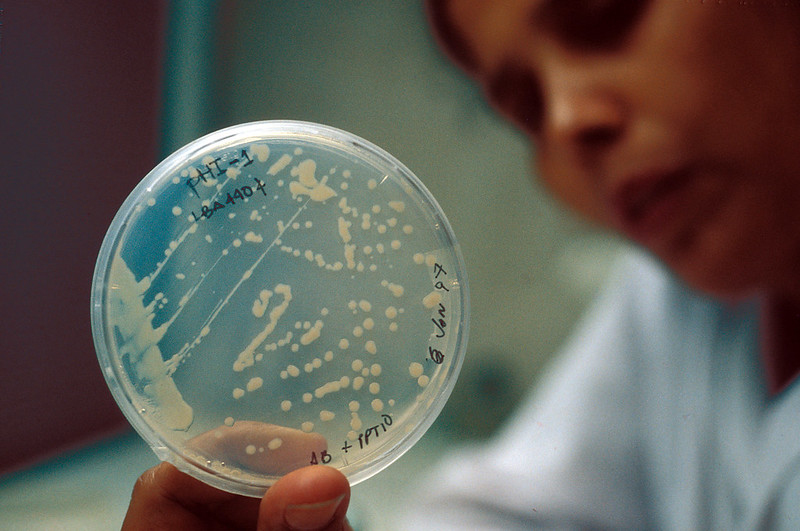
\includegraphics[height=5.3cm]{Kapitel/NGSMotivation/Bilder/typhus_petri.jpg}\\
                    \vspace{0.3cm}\captionof{figure}{Bakterienkulturen in einer Petrischale \cite{typhus_petri}}
                \end{center}
            \end{mdframed}
        \end{textblock}
    }
    \only<4->{
        \begin{textblock}{9.2}(4,3.3)
            \begin{mdframed}[backgroundcolor=white]
                \begin{center}
                    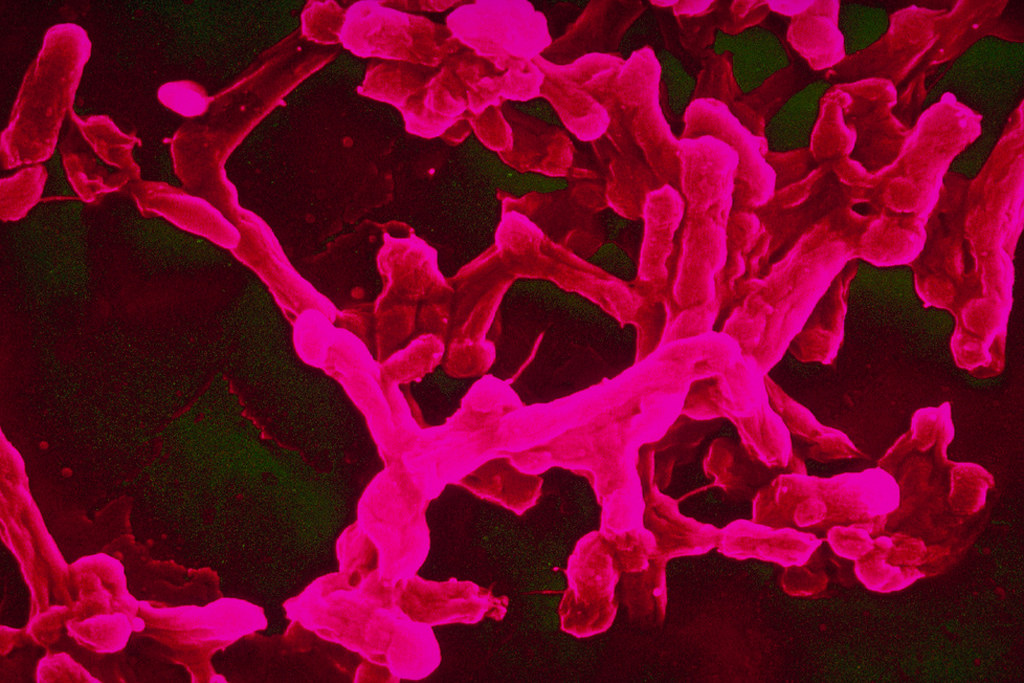
\includegraphics[height=5.3cm]{Kapitel/NGSMotivation/Bilder/typhus_em.jpg}\\
                    \vspace{0.3cm}\captionof{figure}{Elektronenmikroskopische Aufnahme von Typhus-Bakterien \cite{typhus_em}}
                \end{center}
            \end{mdframed}
        \end{textblock}
    }
    \only<5->{
        \begin{textblock}{9.2}(5,3.4)
            \begin{mdframed}[backgroundcolor=white]
                \begin{center}
                    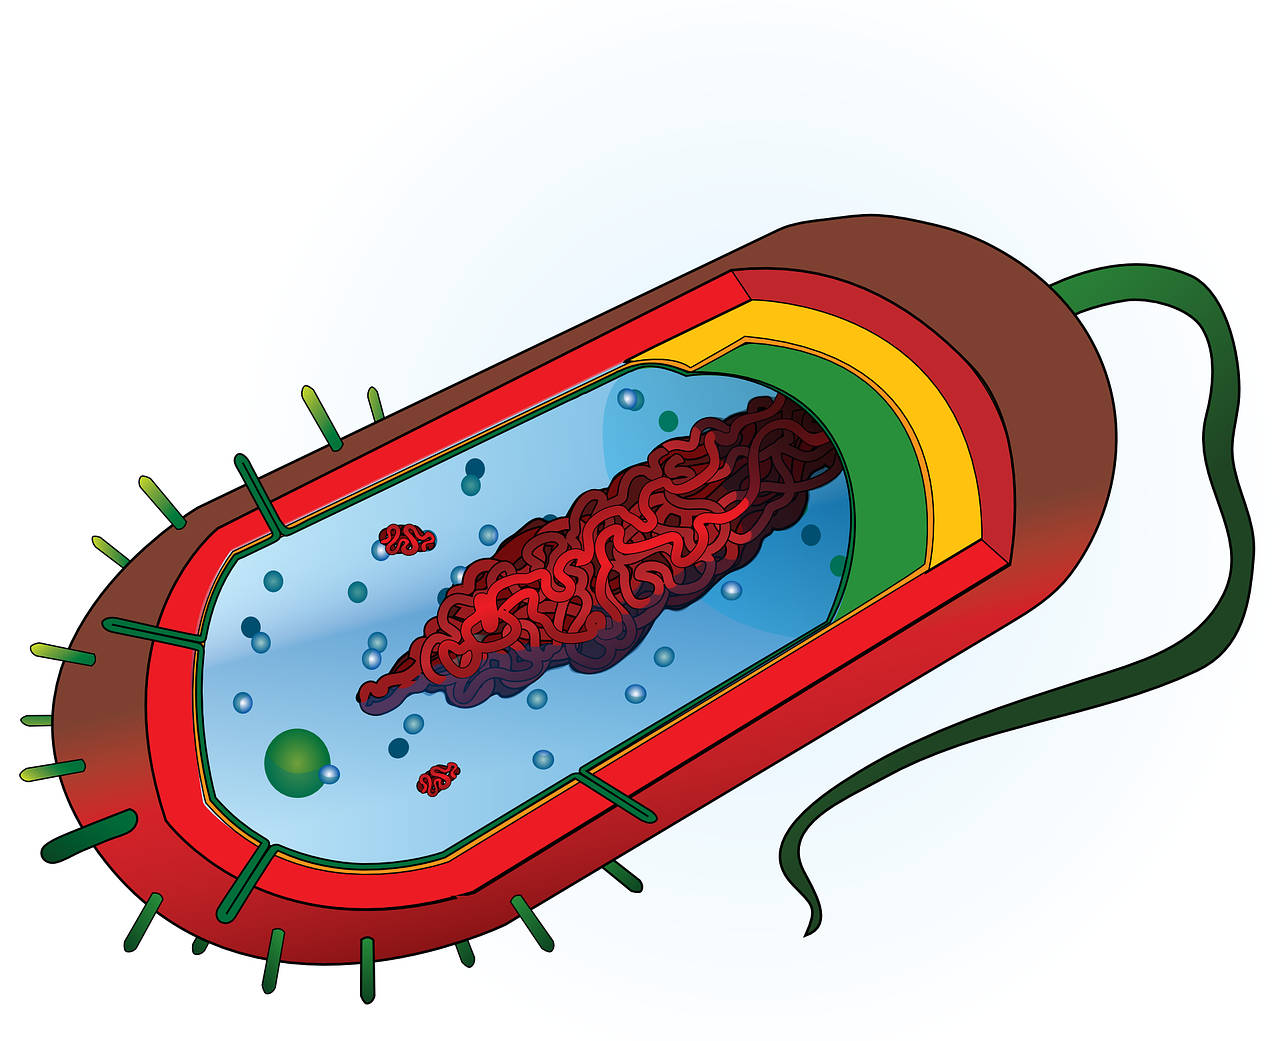
\includegraphics[height=5.3cm]{Kapitel/NGSMotivation/Bilder/bacterium.jpg}\\
                    \vspace{0.3cm}\captionof{figure}{Schematische Darstellung eins Bakteriums \cite{bacterium}}
                \end{center}
            \end{mdframed}
        \end{textblock}
    }
    \only<6->{
        \begin{textblock}{9.2}(6,3.5)
            \begin{mdframed}[backgroundcolor=white]
                \begin{center}
                    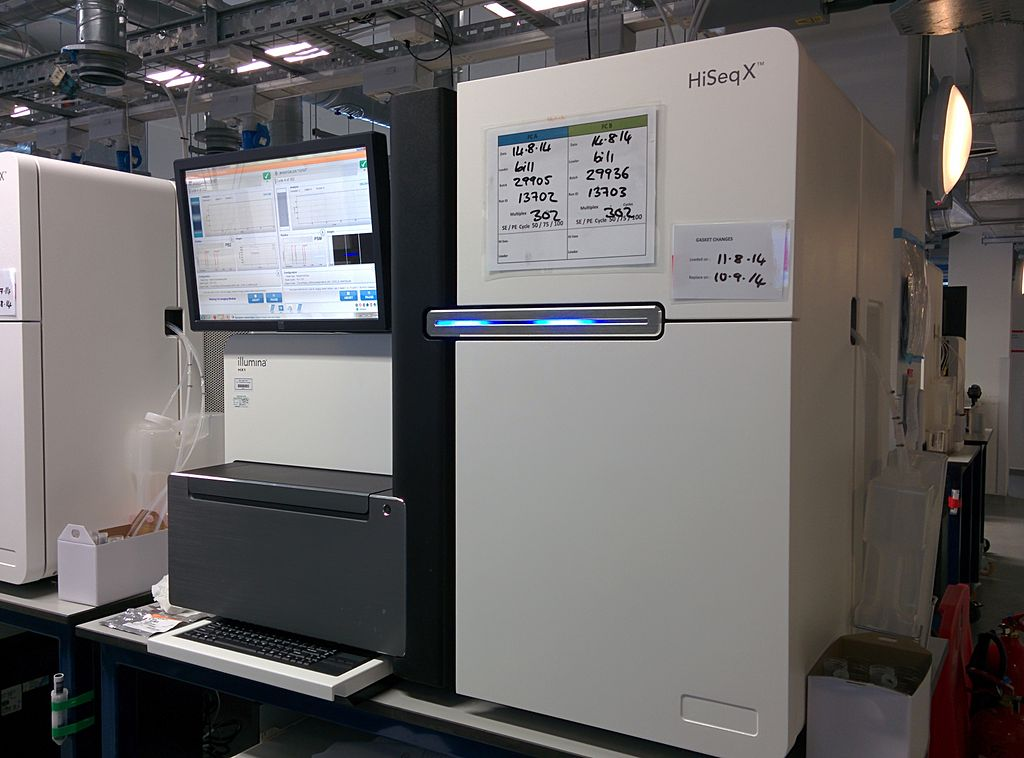
\includegraphics[height=5.3cm]{Kapitel/NGSMotivation/Bilder/hiseq.jpg}\\
                    \vspace{0.3cm}\captionof{figure}{Ein aktuelles Next Generation Sequencing-Gerät \cite{hiseq}}
                \end{center}
            \end{mdframed}
        \end{textblock}
    }
    \only<7->{
        \begin{textblock}{8.9}(7,3.6)
            \begin{mdframed}[backgroundcolor=white]
                \begin{center}
                    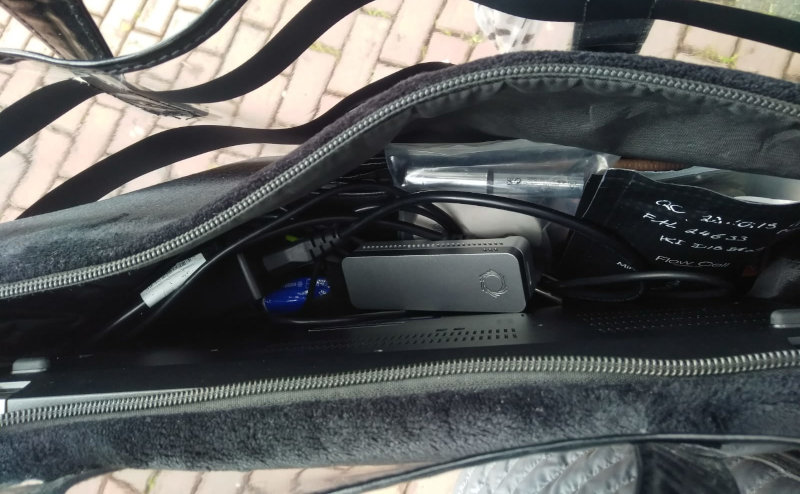
\includegraphics[height=4.8cm]{Kapitel/NGSMotivation/Bilder/minion.jpg}\\
					\vspace{0.3cm}\captionof{figure}{3rd generation NGS-Gerät in Handtasche.}
                \end{center}
            \end{mdframed}
        \end{textblock}
    }
\end{frame}

\begin{frame}{Die Herausforderung}
    \only<1->{
        \begin{textblock}{9.2}(1,3)
            \begin{mdframed}[backgroundcolor=white]
                \begin{center}
                    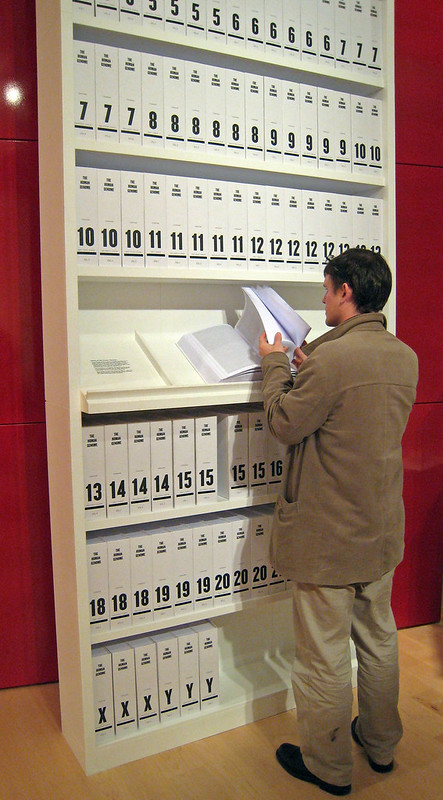
\includegraphics[height=5.2cm]{Kapitel/NGSMotivation/Bilder/problem1.jpg}\\
                    \vspace{0.3cm}\captionof{figure}{Das humane Genom ausgedruckt\cite{problem1}}
                \end{center}
            \end{mdframed}
        \end{textblock}
    }
    \only<2->{
        \begin{textblock}{9.2}(2,3.1)
            \begin{mdframed}[backgroundcolor=white]
                \begin{center}
                    
\includegraphics[height=5.2cm]{Kapitel/NGSMotivation/Bilder/problem2.jpg}\\
                    \vspace{0.3cm}\captionof{figure}{Ein Comic-Heft als Veranschaulichung des Größenverhältnisses von humanem zu Krankenerreger-Genom\cite{problem2}}
                \end{center}
            \end{mdframed}
        \end{textblock}
    }
    \only<3->{
        \begin{textblock}{9.2}(3,3.2)
            \begin{mdframed}[backgroundcolor=white]
                \begin{center}
                    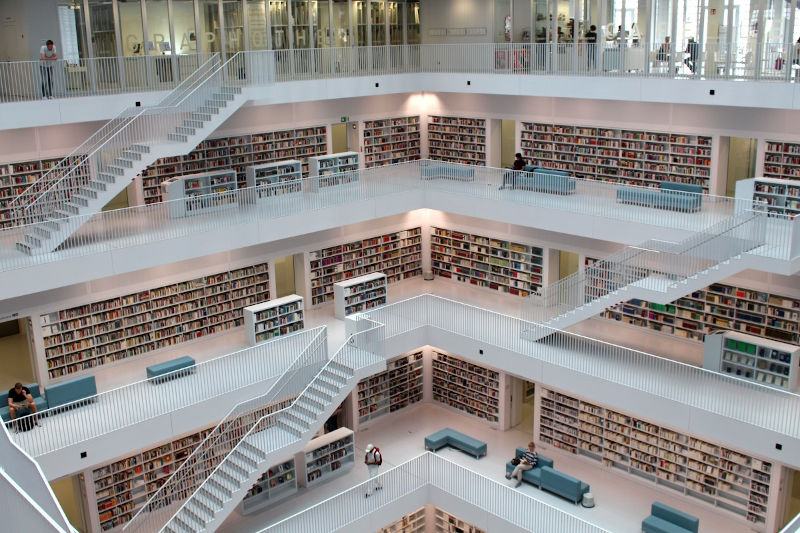
\includegraphics[height=5.2cm]{Kapitel/NGSMotivation/Bilder/library.jpg}\\
                    \vspace{0.3cm}\captionof{figure}{Bild einer Bibliothek\cite{library}}
                \end{center}
            \end{mdframed}
        \end{textblock}
    }
    \only<4->{
        \begin{textblock}{9.2}(4,3.3)
            \begin{mdframed}[backgroundcolor=white]
                \begin{center}
                    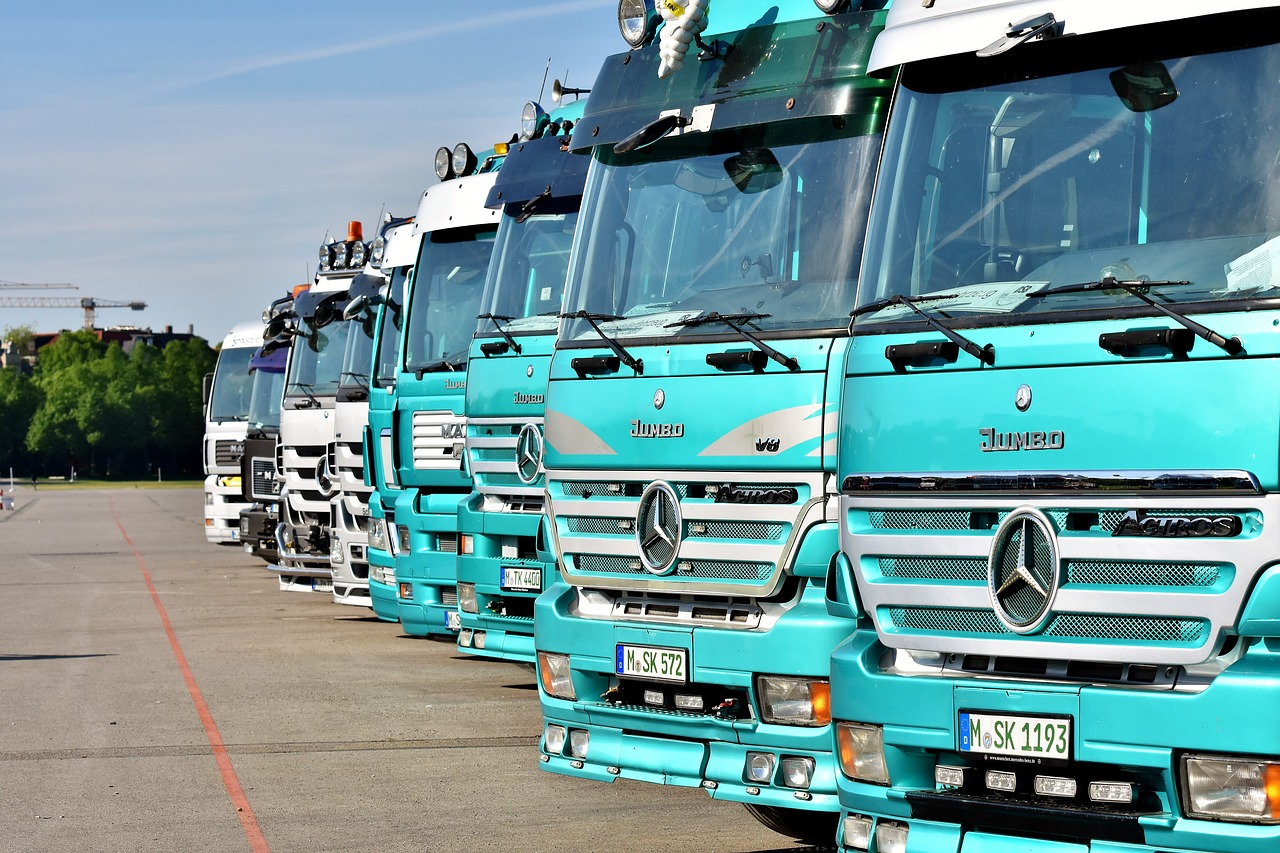
\includegraphics[height=5.2cm]{Kapitel/NGSMotivation/Bilder/problem3.jpg}\\
                    \vspace{0.3cm}\captionof{figure}{LKW-Flotte - das bräuchte man, um die ausgedruckten Sequenzen eines NGS-Laufes zu transportieren\cite{problem3}}
                \end{center}
            \end{mdframed}
        \end{textblock}
    }
    \only<5->{
        \begin{textblock}{9.2}(5,3.4)
            \begin{mdframed}[backgroundcolor=white]
                \begin{center}
                    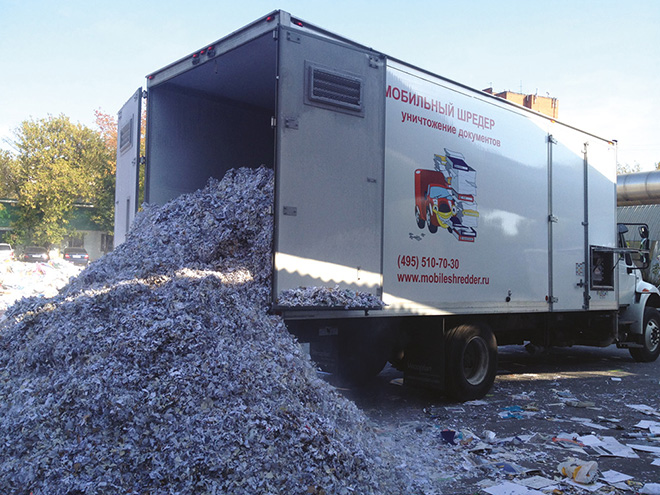
\includegraphics[height=5.2cm]{Kapitel/NGSMotivation/Bilder/problem4.jpg}\\
                    \vspace{0.3cm}\captionof{figure}{Industrieschredder - das, was beim Next Generation Sequencing mit dem Genom passiert \cite{problem4}}
                \end{center}
            \end{mdframed}
        \end{textblock}
    }
    \only<6->{
        \begin{textblock}{10}(6,3.5)
            \begin{mdframed}[backgroundcolor=white]
                \begin{center}
                    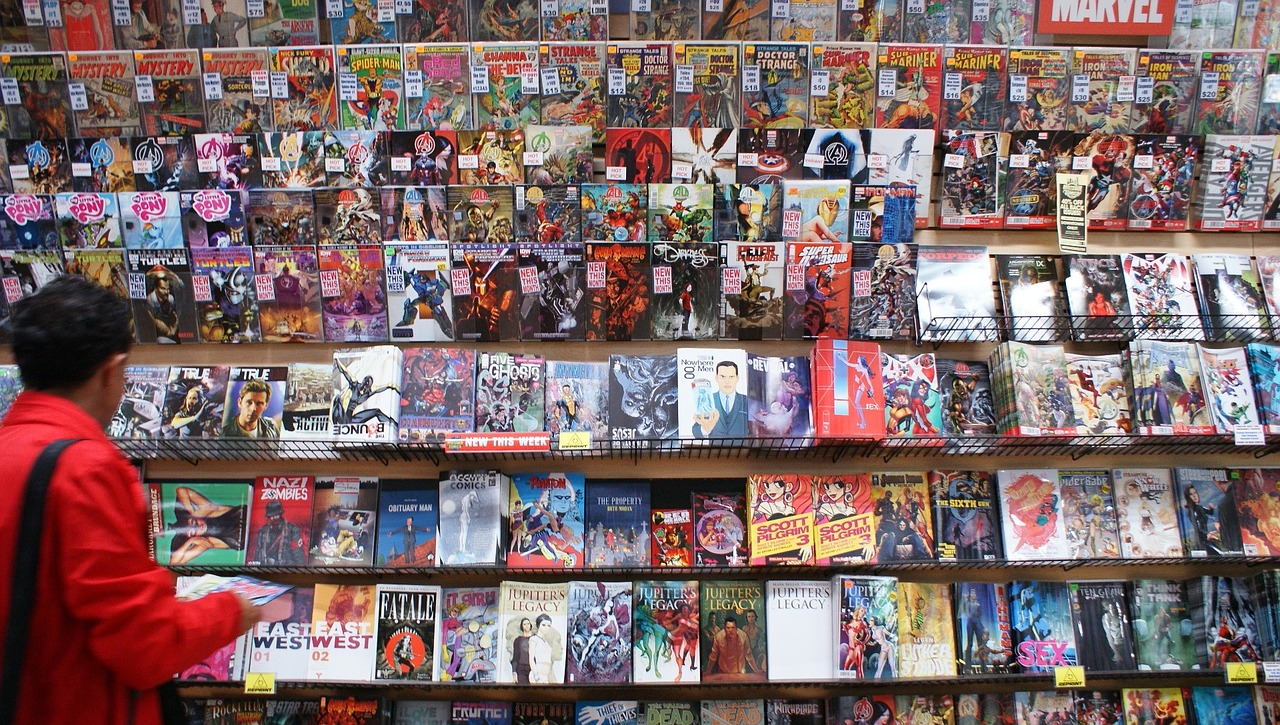
\includegraphics[height=5.2cm]{Kapitel/NGSMotivation/Bilder/problem5.jpg}\\
                    \vspace{0.3cm}\captionof{figure}{Krankheitserreger sind noch vielfältiger als Comic-Hefte\cite{problem5}}
                \end{center}
            \end{mdframed}
        \end{textblock}
    }
\end{frame}
